\section{The Paṇḍaka}

\subsection{The Paṇḍaka in the Pāli and Chinese Vinayas}
The first thing that is striking when comparing the various Chinese schools is that there is no clear consistent term that denotes the {\em paṇḍaka}. The Mahāsaṅghika and Sarvāstivāda Vinaya use the term 種不能男 (impotent lit. incapable of producing seed) in the descriptions in the first Khandhaka on ordination. In the Dharmaguptaka Vinaya this term is only used in the description of the 'half-moon' {\em paṇḍaka}. The term 黃門 ('eunuch') is used in the Dharmaguptaka and Mahīśāsaka Vinaya while in the Sarvāstivāda Vinaya the term is used everywhere but in the ordination Khandhaka. As both the terms 種不能男 (impotent) and 黃門 ('eunuch') are used in the same way in different schools, we can assume that both can denote {\em paṇḍaka} but that the difference in terms point to historical changes in understanding and translation\footnote{Shinsan text X44 0744 0432c13 (四分律名義標釋 第4卷) links both terms, see above.}.

The translation 'eunuch' is a later interpolation due to the etymological development of the Chinese 黃門, meaning 'yellow gate' and derived from the palace eunuchs in the Early Han Dynasty,\footnote{The word 黃門 is translated as 'eunuch' but the characters spell a different word, namely 'yellow gate'. The etymology of the word can be traced back to the Han Dynasty. See Shinsan text X44 0744 0432c09–0433a01: 此翻黃門。阿毗曇。譯為閹人。以無男根故。"This is a 黃門. Translated as castrated man. Because he has no male roots/faculty." This tells the story of the imperial ruler who appointed eunuchs to work for him. Yellow is the color of the middle in the 'Five Directions' and of the earth in the 'Five Elements' and therefore stands for imperial power and state. The color is only used by the emperor and others are not allowed to wear it. Therefore, the palace of the emperor is called the 'Yellow Gate'. In the Easter Han Dynasty, the emperor hired eunuchs and they held rather powerful positions as palace guards, scribes and other official functions. They were called the 'yellow gates'. It is a long story but the eunuchs became very powerful and eventually caused the downfall of the Han Dynasty (see \href{https://en.wikipedia.org/wiki/Han_dynasty}{Wikipedia}). So 'yellow gate' became a synonym for 'eunuch'.} while the word 'impotent' seems to be an earlier interpretation and we also find this back in in the Vedic scriptures\footnote{see \cite{zwilling} page 363–364}. The Chinese culture was vastly different from the Indian culture and I suspect that their own palace eunuchs were the only thing they could relate to as an explanation of the term {\em paṇḍaka}.

The following table compares the description of the various schools, adding the Sanskrit\footnote{Abhidharmakośavyākhyā-Skt: 94, 15–25} and Tibetan\footnote{Abhidharmakośavyākhyā-Tib: D, vol. gu, 85b6–86a3; P, vol. cu, 97b2–7} for reference\footnote{See \href{http://www.itlr.net/hwid:281142}{itlr.net} for details as well a more complete listing of possible meanings and occurrences of these terms}.

\bigskip
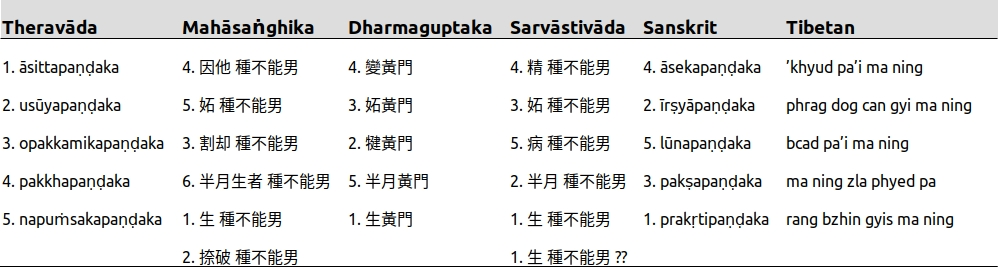
\includegraphics[width=\linewidth]{pandaka.jpg}
% \captionof{figure}{Types of {\em paṇḍaka} in the various Buddhist schools}
\label{pandaka}
\medskip

It is striking that the Dharmaguptaka Vinaya continues to describe several types of castrated men but does not equate these to {\em paṇḍaka}, while the word used for {\em paṇḍaka} is 黃門 (i.e. 'eunuch'), which is the exact definition of a castrated man.

The Theravāda and Mahīśāsaka Vinaya agree on both the background story and do not mentioning a list of types of {\em paṇḍaka}, but the five types of {\em paṇḍaka} are described in the commentaries. The other Vinayas all have a list of {\em paṇḍaka} who are not allowed to ordain but some of these types differ from each other or seem to have a different description. Bhikkhu Sujato\footnote{\cite{sujato2009} page 216–217} also observes that there are various terms where "... a statement on the matter is found explicitly in all or most of the mainland Vinayas, while the Pali canon is silent, and the judgment is found in the commentary." He therefore concludes that there is an obvious explanation for this pattern, namely that the Pāli is earlier.

It is therefore likely that at the time when the five types of {\em paṇḍaka} were introduced, the Theravāda and Mahīśāsaka Vinaya were already closed and therefore these five types appear in the commentarial text instead\footnote{Although the {\em Samantapāsādikā} is attributed to Buddhaghosa in the 5th century CE, this was based on earlier ones, now lost, in Prakrit and Sinhala, which were written down at the same time as the Canon, in the last century BCE. As we see here, some material in the commentaries is found in canonical texts of other schools, suggesting an early common source.}. 

The {\em Śāriputraparipṛcchā} attributes the schism of the Mahāsaṅghika school with the other schools at around 150 BCE to an attempt to expand the Vinaya by the other schools\footnote{See \cite{sujato2012} for a detailed analysis of the history of the various schools}. I therefore conclude that the inclusion of the five types of {\em paṇḍaka} happened before this schism but was not originally in the Vinaya.

The fact that the descriptions of the five terms do not always seem to match seamlessly between schools and that there is some confusion over the term 'impotent', seemingly also denoting those who are socially impaired from marriage (i.e. the concubine's son) as well as the different description of a castrated man in both the Dharmaguptaka and Mahīśāsaka Vinaya seems to point to some ambiguity as to the meaning of {\em paṇḍaka} and the inclusion of the five types could have been an attempt to resolve this.

Considering that the word {\em paṇḍaka} does not appear in any of the early suttas\footnote{The word is not found in any of the early Buddhist Suttas, nor does it appear in the {\em pātimokkhas}, the lists of rules for monastics. Next to the Pāli Vinaya, it appears twice in the {\em Aṅguttara Nikāya}, but both of these only have parallels to the Vinaya or later texts.}, it seems clear that the inclusion of the word in the Vinaya did not happen in the Buddha's lifetime but was added later, possibly as a result of the discussions with the Brahmins and Jains, for whom the {\em paṇḍaka} could not ordain.

In \ref{appendix2}, \ref{pali1} and \ref{sanskrit1} I have charted the occurances of the various words throughout the Pāli and Sanskrit texts. This illustrates that the {\em paṇḍaka} only occurs in the Vinaya and Commentaries in the Pāli. The Sanskrit texts in this graph are not entirely organised by lateness but it is clear that the {\em paṇḍaka} mainly appears in the Vinaya and {\em Śāstrapiṭaka}. The {\em klība} is notable by it's absense in the Buddhist texts in \ref{sanskrit1} and only appears in the Vedic and later Brahmanical texts. It does not appear in the Pāli texts at all. One explanation for this might be that the terms {\em klība} and {\em paṇḍaka} have been mixed up because their meanings were at least in part overlapping. What is also striking is that the umbrella term {\em napuṃsaka} only appears in the Pāli commentarial texts and not in any of the earlier collections. It is however a recurrent term in the Vedic and Brahmanical texts. We also see that this term becomes more prominent in the later Anya commentaries as well as in the Brahmanical {\em Śāstra} collections, which points to a shift in emphasis, and possibly meaning, of this term in later times at the expense of the prominence of {\em paṇḍaka}. As these are later texts I have not looked into them in great details and this might be an interesting topic for later studies.

\subsection{History}
After having looked at the references and descriptions of the word {\em paṇḍaka} in Vedic text, Jain discussions and Buddhist scriptures of both Pāli and Chinese origin, a clearer picture emerges of what the {\em paṇḍaka} really is and the reasons behind the Buddhist rules against ordination.

As we have seen in the previous chapter the oldest emergence of the {\em paṇḍaka} and the {\em klība} as sub-categories of the {\em napuṃsaka} ('neither male nor female') happened in Vedic times. They are the 'un-males', the 'impotent', destined from birth to play a role in the larger fabric of Indian religion, society and culture. They are the embodiment of the feminine in the masculine, a living myth. They are categorised by their feminine behavior and dress, their impotence, their occupation as religious dancers and singers and their emasculation. They are there to remind us of the deeply ambivalent attitude of men towards women and women's sexuality, their desire for, and at the same time their fear of the feminine. Allan Bomhard\footnote{\cite{bomhard}} points out that the word can be a loan-word from the Dravidian {\em peṇṭan, peṇṭakan, peṇṭakam}, which can mean both hermaprodite and eunuch. This is interesting because it is clear that at least in Dravidian no difference is made between a eunuch and a hermaphrodite and I believe that the way we need to see the {\em paṇḍaka} is indeed as both these terms, namely an emasculated male who has female characteristics ({\em liṅga}).

With the emergence of the Jain ascetics a debate started with regards to the position of women in the order, and as a consequence the position of the {\em napuṃsaka}. This discussion necessitated the identification of the characteristics that make up a male, a female and by consequence a {\em napuṃsaka}. We see that a similar discussion was held among the Buddhists\footnote{\cite{sujato2009}}, especially after the Buddha himself passed away and the order found itself without a leader. This discussion was also fuelled by the public opinion of the celibate monastics. We know from both the Buddhist Suttas as the Jain scriptures that debates were also held between the Jains and Buddhists about a variety of subjects and no doubt there was an influence between these orders\footnote{\cite{sujato2009} page 54–55 points out that various rules that seem out of place in Buddhist scriptures appear in the Jain texts, even using identical wording at times.}. Although the Jain order is older, their scriptures were written down much later so it is difficult to determine who borrowed from whom. What is clear however is that they borrowed from each other. As a rule of thumb we can say that if something seems out of place in the Buddhist scriptures in the light of the Dhamma taught in the overall canon and it is found elsewhere in Jain or other Indic texts, there is a fair chance that this does not originate from the Buddha himself.

As a result the Buddhist Vinaya was redacted during the Second Council. It is not so far-fetched to infer that if the Vinaya was redacted with regards to women's ordination, the position of the {\em paṇḍaka} was also laid down at this time. This is when we see the emergence of the {\em paṇḍaka} as the hyperlibidous effeminate male who seduces monks and lay men alike, who is unable to maintain his precepts and who can, by his very nature, not be a monk. This idea of the hyperlibidousness of the {\em paṇḍaka} because he possesses both male and female {\em veda} we have also seen in the Jain scriptures. But there is no further explanation of what the {\em paṇḍaka} really is and what his characteristics are until later, when the five types of {\em paṇḍaka} are defined. 

At this point in time the Jain and Buddhist scriptures and their development begin to diverge as schools begin to emerge after King Ahsoka has sent his missionaries to different parts of his empire. The Jain also begin to create subdivisions of the {\em napuṃsaka}, but here the {\em paṇḍaka} is not further divided and remains as a person who cannot ordain. 

The Buddhist scriptures are dispersed and eventually translated into Chinese in the various schools. There the word {\em paṇḍaka} was first translated as 'impotent' (種不能男) and later as 'eunuch' (黃門). The translation 'eunuch' however was taken from the word 'yellow gate', denoting the Han Dynasty imperial palace eunuchs. This was possibly the only way that the Chinese could relate to a {\em paṇḍaka}, being unfamiliar with the rich religious concept that they embody. It is clear that the Chinese palace eunuchs cannot be compared to the hijra from India.

\begin{figure}[!tbp]
  \begin{subfigure}{0.4\textwidth}
    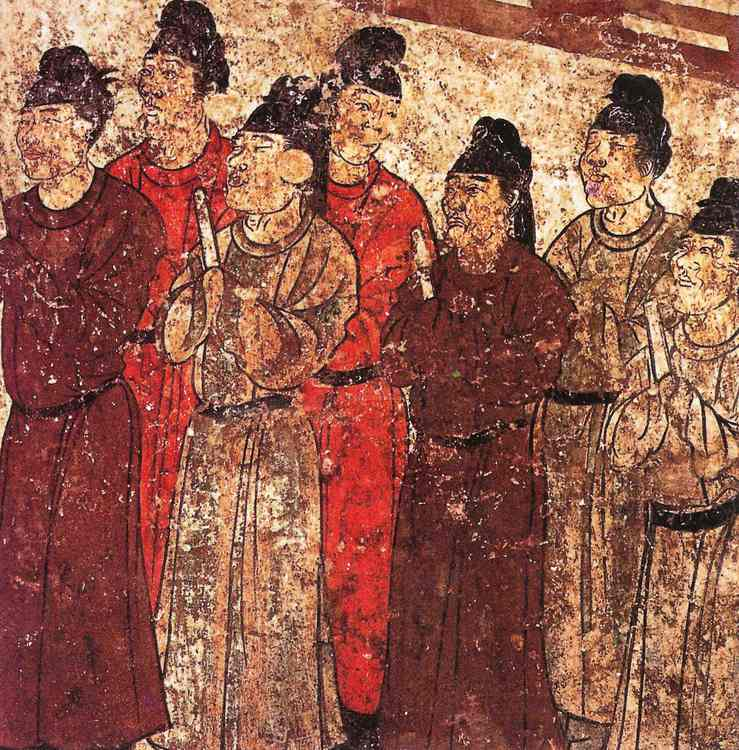
\includegraphics[width=\textwidth]{Eunuchs-in-ancient-China.jpg}
    \caption{Palace eunuchs in ancient China}
  \end{subfigure}
  \hfill
  \begin{subfigure}{0.4\textwidth}
    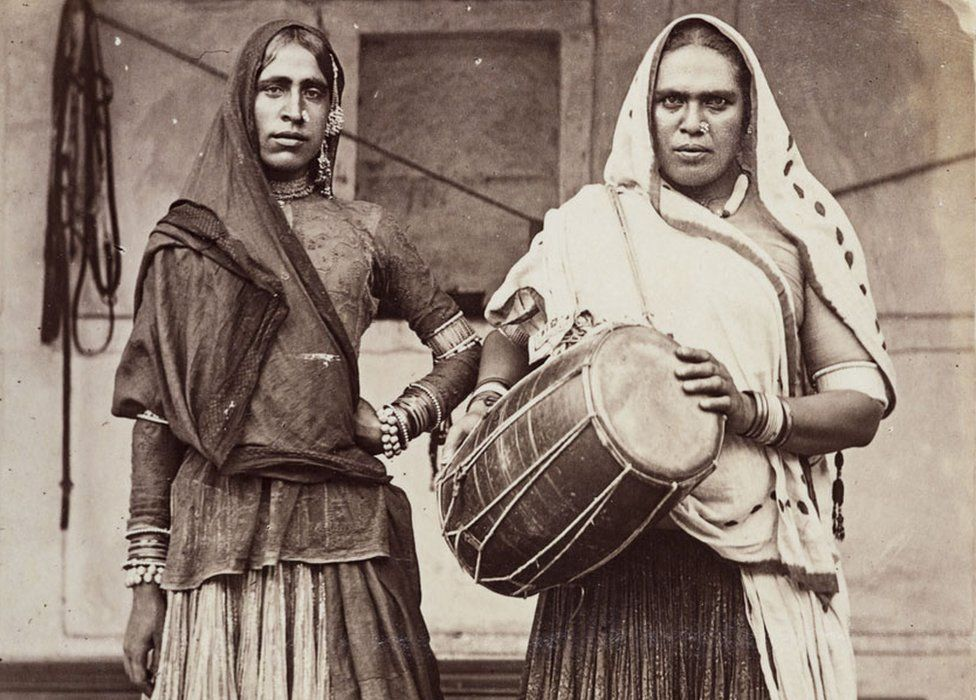
\includegraphics[width=\textwidth]{hijra.jpg}
    \caption{Hijra in India}
  \end{subfigure}
\end{figure}

\subsection{The Five Types}
The castrated {\em paṇḍaka} i.e. a eunuch, is only one type of the five types that cannot ordain, which makes it highly unlikely that the word {\em paṇḍaka} means 'eunuch'. We would also not expect a eunuch to have hyperlibidousness. After all, castrated men were often employed as harem guards just for the reason that they are no longer interested in sexual activity and therefore considered safe. Moreover, the Dharmaguptaka Vinaya treats the castrated man as something other than a {\em paṇḍaka}.

To fully understand the types of {\em paṇḍaka} in the scriptures, we have to look again at the understanding of the gender roles at that time. Whether or not the {\em paṇḍaka} in form of the religious embodiment of the feminine in the masculine was already engaged in prostitution at the time of the Buddha or not, in any case he was seen to have the female {\em veda} simply because he was 'not a male'. He dressed and behaved like a woman, a temptress that could arouse desire in the celebate monk. 

As we have seen in the Jain scriptures, the discussion to overcome the ambiguities in the understanding of the word {\em paṇḍaka} resulted over time in changes in meaning and use and the definition of sub-categories. I believe that it is likely that the term {\em opakkamikapaṇḍaka} represented a castrated man, the {\em klība}, or the initiated hijra, while the {\em napuṁsakapaṇḍaka} was the re-definition of the original {\em paṇḍaka}, the still uninitiated hijra, or the 'female {\em napuṃsaka}' that we saw emerging in the Jain commentarial texts.

The {\em pakkhapaṇḍaka} is interesting and several explations have been given by authors over time, none of which I find convincing. Allan Bomhard\footnote{See \cite{bomhard}} advocates that the word {\em pakkha} should not be translated as 'half moon' but that the meaning of the word is something like a sex-addict. I refute this argument because the characters used to denote this type of pandaka in the Chinese Vinayas of all schools are 半月, which literally means 'half moon'. It is also mentioned in various Chinese commentarial texts\footnote{f.i. X44 0744 0432c17 四分律名義標釋} that the 'half moon' is 'not a male' and thus a form of {\em napuṃsaka} for half of the month and the other half he is a male. All texts are consistent in this. As we can still understand the meaning of the other four categories and understand their meaning in light of people's physiology or sexual fetishes, the 'half-moon' {\em paṇḍaka} is an enigma. Turning back to the Vedic texts however, we find in the {\em Uttarakanda} of the {\em Rāmāyaṇam}\footnote{Rām 7.78–79. See also \cite{goldman} page 379–380} the story of King Ila. In this epic tale the king accidentally stumbles upon the Goddess Pārvatī in intimate embrace with Śiva, who turn him into a woman. Now Ilā, she turns to the Goddess for mercy to restore her manhood but is only granted half her wish; namely that she has to change sex each month. With the change of sex also comes a change in sexual desire. As a woman she falls in love, becomes pregnant and gives birth, reverting back and forth between male and female. The theme of changing genders based on the phases of the moon is a recurrent theme in the Vedic myths and it is not unlikely that this mythical theme has found its way into the Vinaya in the form of the {\em pakkhapaṇḍaka}. After all, another rule in the Vinayas of all the schools tells the tale of a shape-shifting serpent, a mythological beast, a {\em Nāga}\footnote{Khandhaka 1 Pabbajjā PTS vol 1 page 86-88}, who ordains as a monk, is later discovered and a new rule is laid down in much the same manner as for the {\em paṇḍaka}, barring him and all his kind from ordination. The fabric of myth and reality can easily overlap in Indic culture. The Vinaya is full of various strange and wonderful beings. The ­{\em Bhikkhu Pā­rāji­ka} 1, the rule against sexual intercourse, mentions that a monk is not allowed to have sex with a list of beings, namely a dragon, a spirit, a ghost and a {\em paṇḍaka}\footnote{PTS vol. 3 page 37: {\em Tena kho pana samayena aññataro bhikkhu nāgiyā methunaṃ dhammaṃ paṭisevi … yakkhiniyā methunaṃ dhammaṃ paṭisevi … petiyā methunaṃ dhammaṃ paṭisevi … paṇḍakassa methunaṃ dhammaṃ paṭisevi. Tassa kukkuccaṃ ahosi … pe … “āpattiṃ tvaṃ, bhikkhu, āpanno pārājikan”ti.}}. The fact that the {\em paṇḍaka} is listed in a list of mythological beings is indicative of its orgins and how they were viewed at that time. We find similar lists in the other Vinayas.

As for the other two, the {\em āsittapaṇḍaka} and the {\em usūyapaṇḍaka}, who at least in the Theravāda tradition are allowed to ordain, I believe they embody another of the Jain categories, namely the category of the {\em puruṣanapuṃsaka} (male {\em napuṃsaka}). Although they might be impotent and are therefore also in possession of the female {\em veda}, they can "pass" as a man an therefore not only appear as men to the lay supporters but also to the celibate monks they live with who are not arroused by their presence. The relaxation of the rules for these two types also runs parallel with the development in the Jain scriptures. But unlike the Jain, no further abolishment of this entire rule against the ordination of {\em paṇḍaka} was reached simply because the Buddhist scriptures were closed while the Jain scriptures continued to evolve for many centuries thereafter.

\subsection{Meaning}
The {\em paṇḍaka} does not allow itself to be reduced to a mere word to make it acceptable and understandable for the rational mind. As Serena Nanda\footnote{\cite{nanda} page 20} argues: "Whereas Westerners feel uncomfortable with the ambiguities and contradictions inherent in such in-between categories as transvestism, homosexuality, hermaphroditism, and transgenderism, and make strenuous attempts to resolve them, Hinduism not only accommodates such ambiguities, but also views them as meaningful and even powerful." It is the divine representation of the feminine within the masculine. It is the human representation of the mythical tales which have deep psychological roots, namely the ambivalence that leads to the inner struggle between man's love of the feminine and his fear thereof. The {\em paṇḍaka} does not match any contemporary notions. If we have to capture the {\em paṇḍaka} in one word, it would be 'hijra'. The hijra is a man, impotent from birth, emasculated in an initiation ritual, part of a caste, a religious seeker enacting the feminine of Śiva by dressing and behaving in traditional women's gender roles, changing into it and feeling the feminine sexual desire for the masculine.
